\documentclass[
  bibliography=totoc,     % Literatur im Inhaltsverzeichnis
  captions=tableheading,  % Tabellenüberschriften
  titlepage=firstiscover, % Titelseite ist Deckblatt
]{scrartcl}

% Paket float verbessern
\usepackage{scrhack}

% Warnung, falls nochmal kompiliert werden muss
\usepackage[aux]{rerunfilecheck}

% unverzichtbare Mathe-Befehle
\usepackage{amsmath}
% viele Mathe-Symbole
\usepackage{amssymb}
% Erweiterungen für amsmath
\usepackage{mathtools}

% Fonteinstellungen
\usepackage{fontspec}
% Latin Modern Fonts werden automatisch geladen
% Alternativ:
%\setromanfont{Libertinus Serif}
%\setsansfont{Libertinus Sans}
%\setmonofont{Libertinus Mono}
\recalctypearea % Wenn man andere Schriftarten gesetzt hat,
% sollte man das Seiten-Layout neu berechnen lassen

% deutsche Spracheinstellungen
\usepackage{polyglossia}
\setmainlanguage{german}


\usepackage[
  math-style=ISO,    % ┐
  bold-style=ISO,    % │
  sans-style=italic, % │ ISO-Standard folgen
  nabla=upright,     % │
  partial=upright,   % ┘
  warnings-off={           % ┐
    mathtools-colon,       % │ unnötige Warnungen ausschalten
    mathtools-overbracket, % │
},                       % ┘
]{unicode-math}

% traditionelle Fonts für Mathematik
\setmathfont{Latin Modern Math}
% Alternativ:
%\setmathfont{Libertinus Math}

\setmathfont{XITS Math}[range={scr, bfscr}]
\setmathfont{XITS Math}[range={cal, bfcal}, StylisticSet=1]

% Zahlen und Einheiten
\usepackage[
locale=DE,                   % deutsche Einstellungen
separate-uncertainty=true,   % immer Fehler mit \pm
per-mode=symbol-or-fraction, % / in inline math, fraction in display math
]{siunitx}

% chemische Formeln
\usepackage[
version=4,
math-greek=default, % ┐ mit unicode-math zusammenarbeiten
text-greek=default, % ┘
]{mhchem}

% richtige Anführungszeichen
\usepackage[autostyle]{csquotes}

% schöne Brüche im Text
\usepackage{xfrac}

% Standardplatzierung für Floats einstellen
\usepackage{float}
\floatplacement{figure}{htbp}
\floatplacement{table}{htbp}

% Floats innerhalb einer Section halten
\usepackage[
section, % Floats innerhalb der Section halten
below,   % unterhalb der Section aber auf der selben Seite ist ok
]{placeins}

% Seite drehen für breite Tabellen: landscape Umgebung
\usepackage{pdflscape}

% Captions schöner machen.
\usepackage[
  labelfont=bf,        % Tabelle x: Abbildung y: ist jetzt fett
  font=small,          % Schrift etwas kleiner als Dokument
  width=0.9\textwidth, % maximale Breite einer Caption schmaler
]{caption}
% subfigure, subtable, subref
\usepackage{subcaption}

% Grafiken können eingebunden werden
\usepackage{graphicx}
% größere Variation von Dateinamen möglich
\usepackage{grffile}

% schöne Tabellen
\usepackage{booktabs}

% Verbesserungen am Schriftbild
\usepackage{microtype}

% Literaturverzeichnis
\usepackage[style=alphabetic,]{biblatex}
% Quellendatenbank
\addbibresource{lit.bib}
\addbibresource{programme.bib}

% Hyperlinks im Dokument
\usepackage[
  unicode,        % Unicode in PDF-Attributen erlauben
  pdfusetitle,    % Titel, Autoren und Datum als PDF-Attribute
  pdfcreator={},  % ┐ PDF-Attribute säubern
  pdfproducer={}, % ┘
]{hyperref}
% erweiterte Bookmarks im PDF
\usepackage{bookmark}

% Trennung von Wörtern mit Strichen
\usepackage[shortcuts]{extdash}

\title{US2: Scanverfahren in der Ultraschalltechnik}
\author{
  Simon Schulte
  \texorpdfstring{
    \\
    \href{mailto:simon.schulte@udo.edu}{simon.schulte@udo.edu}
  }{}
  \texorpdfstring{\and}{, }
  Tim Sedlaczek
  \texorpdfstring{
    \\
    \href{mailto:tim.sedlaczek@udo.edu}{tim.sedlaczek@udo.edu}
  }{}
}
\publishers{TU Dortmund – Fakultät Physik}


\date{Durchführung: 20.06.2017\\
      Abgabe: 27.06.2017}

\begin{document}

\maketitle
\thispagestyle{empty}
\tableofcontents
\newpage
\setcounter{page}{1}
\section{Zielsetzung}
\label{sec:zielsetzung}
Ziel des Versuchs ist es, verschiedene Scanverfahren zur
Ultraschallechographie kennenzulernen.
\section{Theorie}
\label{sec:theorie}
Als Ultraschall werden die Schallwellen bezeichnet, die eine Frequenz zwischen
\SI{20}{\kilo\hertz} und \SI{1}{\giga\hertz} haben. Ultraschalluntersuchungen
finden vorallem Verwendung in der Medizin. Ultraschall ist natürlich auch
Schall und Schall lässt sich als longitudinale Welle mathematisch als
\begin{equation}
  p(x,t)\,=\,p_0\,+\,v_0 Z \cos(\omega t-kx)
\end{equation}
beschreiben. Hierbei ist $Z$ der Schallkennwiderstand, der sich als $Z=c*\rho$
beschreiben lässt mit der Dichte $\rho$ des durchstrahlten Materials und der
Schallgeschwindigeit $c$, welche durch das betrachtete Material festgelegt wird.
Die Schallgeschwindigkeit einer Flüssigkeit lässt sich durch
\begin{equation}
  c_{Fl}\,=\,\sqrt{\frac{1}{\kappa \cdot \rho}}
  \label{eqn:schallspeed}
\end{equation}
berechnen. Dabei bezeichnet $\kappa$ die Kompressibilität und $\rho$ die Dichte
der Flüssigkeit. Die Schallgeschwindigkeit von Festkörpern lässt sich durch
\begin{equation}
  c_{Fe}\,=\,\sqrt{\frac{E}{\rho}}
  \label{eqn:festkörper}
\end{equation}
berechnen. Dabei bezeichnet $E$ das Elastizitätsmodul und $\rho$ die Dichte des
Festkörpers. Die Analogie zur Schallgeschwindigkeitsberechnung in Flüssigkeiten
ist gegeben durch die Beziehung $E\,\iff \, \kappa^{-1}$. Im Gegensatz zu
Schall in Flüssigkeiten treten beim Schall durch Festkörper sowohl
Longitudinalwellen als auch Transversalwellen auf.
Dabei bezeichnet die Relation
\begin{equation}
  I(x)\,=\,I_0 \cdot e^{\alpha x}
  \label{eqn:intensität}
\end{equation}
die Tatsache, dass die Intensität $I_0$ einer Schallwelle exponentiell mit der
Strecke $x$ abnimmt. Es geht Energie durch Absorption verloren. $\alpha$
bezeichnet dabei den Absorptionskoeffizient der Schallamplitude.
Der Reflexionskoeffizient
\begin{equation}
  R\,=\,\left(\frac{Z_1 - Z_2}{Z_1 + Z_2}\right)^2
  \label{eqn:reflexionskoeffizient}
\end{equation}
gibt das Verhältnis von reflektierter und einfallender Schallintensität an.
Dabei bezeichnet $Z\,=\,\rho \cdot c$ die akustische Impedanz. \\
\\
Um Ultraschall zu erzeugen wird der piezo-elektrische Effekt genutzt. Dabei
wird ein piezoelektrischer Kristall in ein elektrisches Wechselfeld gegeben.
Dadurch werden Schwingungen im Ultraschallbereich angeregt. Es ist auch möglich
den Piezokristall als Empfänger zu nutzen. Dann regen die Schallwellen den
Kristall an. Bei diesen Kristallen sind gleichbleibende physikalische
Eigenschaften sinnvoll. \\
\\
Abbildung \ref{fig:US22} zeigt das Durchschallungsverfahren. Ein
Ultraschallsender sendet einen kurzzeitigen Schallimpuls aus. Dieser wird am
anderen Ende des Probenstücks mit einem Ultraschallempfänger aufgefangen. Diese
Methode bietet den Vorteil, dass sie zwar zuverlässig Fehlstellen im Material
feststellen kann, aber nicht deren genauen Ort vorhersagen.
\begin{figure}[H]
  \centering
  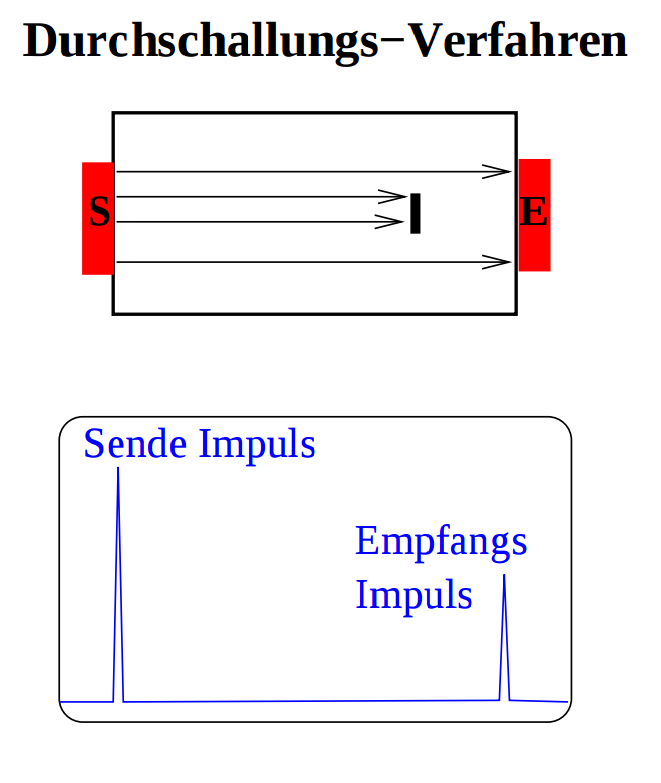
\includegraphics[width=0.5\textwidth]{US22.png}
  \caption{Das Durchschallungsverfahren. \cite{anleitung}}
  \label{fig:US22}
\end{figure}
\noindent
Abbildung \ref{fig:US23} zeigt das Impuls-Echo-Verfahren. Hier wird erneut ein
Schallimpuls von einem Ultraschallsender ausgesendet. Beim
Impuls-Echo-Verfahren wird dieser allerdings an einer Grenzfläche reflektiert
und vom Ultraschallsender wieder aufgenommen. Somit lassen sich auch Aussagen
über die Größe der Fehlstelle machen. Dafür wird die Formel
\begin{equation}
  s\,=\, \frac{1}{2} c t
  \label{eqn:strecke}
\end{equation}
genutzt. Dabei bezeichnet $c$ die Schallgeschwindigkeit in dem jeweiligen
Medium und $t$ die Zeit.
\begin{figure}[H]
  \centering
  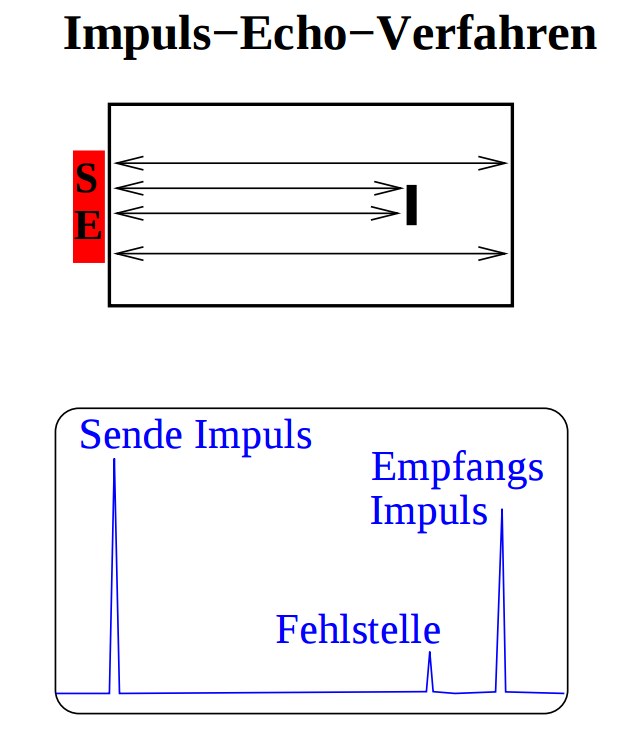
\includegraphics[width=0.5\textwidth]{US23.png}
  \caption{Das Impuls-Echo-Verfahren. \cite{anleitung}}
  \label{fig:US23}
\end{figure}
\noindent
Der Amplituden Scan (A-Scan) stellt die Echoamplituden als Funktion der Zeit
dar. Der A-Scan ist ein eindimensionales Scanverfahren.
Der Brightness Scan (B-Scan) stellt die Echoamplituden in
Helligkeitsabstufungen dar. Der B-Scan ist ein zweidimensionales Scanverfahren.
Dafür muss die Sonde über das zu untersuchende Material bewegt werden.
Der Time-Motion Scan (TM-Scan) kann die Bewegung eines Organs durch eine
schnelle Abtastung aufnehmen.
\section{Versuchsaufbau}
\label{sec:aufbau}
Es werden ein Ultraschallechoskop, eine Ultraschallsonde mit einer Frequenz von
\SI{1}{\mega\hertz} und eine Ultraschallsonde mit einer Frequenz von
\SI{4}{\mega\hertz} verwendet. Diese sind an einen PC angeschlossen, welcher
für die Datenaufnahme und die Datenanalyse verantwortlich ist. Als
Kontaktmittel wird immer bidestilliertes Wasser genutzt.\\
\\
In diesem Versuch wird ein Acrylblock mit verschiedenen Bohrungen genutzt.
Abbildung \ref{fig:US21} zeigt den Aufbau des verwendeten Acrylblocks.
\begin{figure}[H]
  \centering
  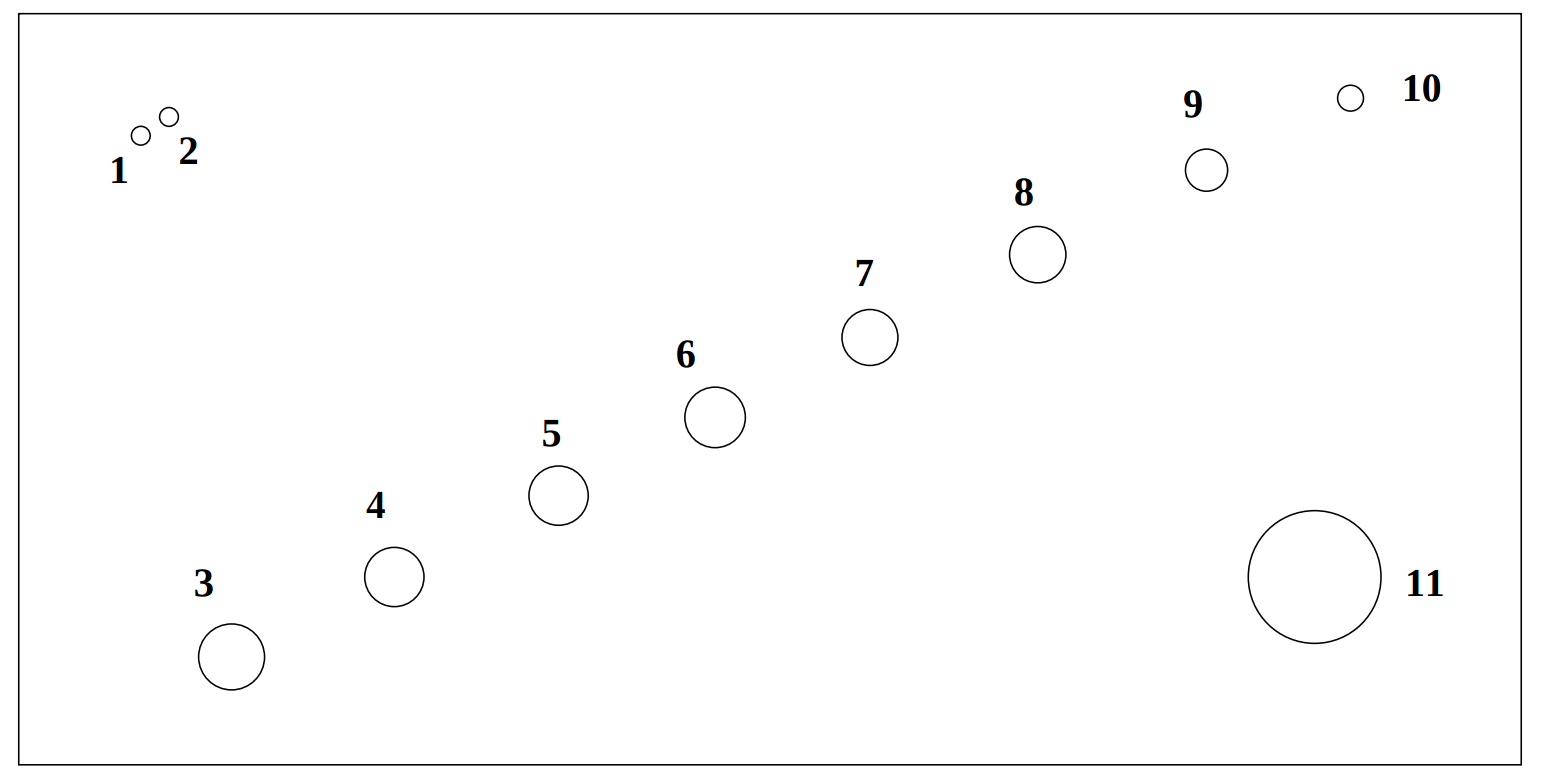
\includegraphics[width=0.7\textwidth]{US21.png}
  \caption{Der Aufbau des Acrylblocks. \cite{anleitung}}
  \label{fig:US21}
\end{figure}
\section{Versuchsdurchführung}
\label{sec:versuchsdurchführung}
Zunächst werden die Abmessungen des verwendeten Acrylblocks mit einer
Schieblehre
bestimmt. Dabei ergeben sich die Werte:
\begin{align*}
  Breite\,=\,\SI{15.025}{\centi\meter} \\
  Tiefe\,=\,\SI{8.04}{\centi\meter} \\
  Dicke\,=\,\SI{4.03}{\centi\meter}.
\end{align*}
Danach wird mit Hilfe des Impuls-Echo-Verfahrens die Lage der Bohrungen im
Acrylblock bestimmt. Dafür wird zunächst etwas destilliertes Wasser auf den
Acrylblock getropft um danach mit einer \SI{1}{\mega\hertz} Sonde den Block zu
untersuchen.
Als nächstes werden die Tiefen der jeweiligen Störstelle bestimmt. Dafür
werden an verschiedenen Stellen mit Hilfe des A-Scans die Schalllaufzeiten
gemessen. Diese Messung wird nach Umdrehen des Acrylblocks wiederholt. Mit
diesen Werten ist es dann möglich die Größen der Störstellen zu bestimmen.
Als nächstes werden die Bohrungen 1 und 2 genauer betrachtet. Mit einem A-Scan
werden diese beiden Bohrungen nun vermessen, um das Auflösungsvermögen zu
untersuchen.\\
\\
Nun wird der Acrylblock mit dem B-Scan untersucht. Es wird erneut der
Acrylblock mit destilliertem Wasser betröpfelt. Dann wird mit der
\SI{4}{\mega\hertz} Sonde der Block untnersucht. Danach wird die Sonde langsam
und konstant über den Acrylblock geführt, um einen genauen B-Scan zu bekommen.
Danach wird der Block umgedreht und die Messung wiederholt. Als letzten Teil
der Untersuchung des Acrylblocks mit dem B-Scan werden aus den erlangten
Bildern die Abmessungen der Störstellen bestimmt. \\
\\
Als letztes wird mit Hilfe des TM-Scans ein Herzmodell untersucht. Das
Herzmodell wird dafür zu etwa einem Drittel mit Wasser befüllt und die Sonde so
positioniert, dass sie grade so einen vollständigen Kontakt zur
Wasseroberfläche hat.
Dann wird die Laufzeit des Echos mit einem A-Scan bestimmt. Dann wird eine
Herzfrequenz simuliert. Diese wird mit einem TM-Scan
aufgenommen. Mit den gemessenen Daten lässt sich dann auch das Herzvolumen
bestimmen.\\
\\
Für die Schallgeschwindigkeiten ergeben sich die Werte:
\begin{align*}
  v_L\,=\,\SI{343}{\meter\per\second} \\
  v_W\,=\,\SI{1450}{\meter\per\second} \\
  v_A\,=\,\SI{2730}{\meter\per\second}.
\end{align*}
Dabei bezeichnet $v_L$ die Schallgeschwindigkeit in der Luft, $v_W$ die
Schallgeschwindigkeit in destilliertem Wasser und $v_A$ die
Schallgeschwindigkeit in Acryl.
\section{Fehlerrechnung}
\label{sec:fehlerrechnung}
Die in der Auswertung verwendeten Mittelwerte mehrfach gemessener Größen sind gemäß der
Gleichung

\begin{equation}
    \bar{x}=\frac{1}{n}\sum_{i=1}^n x_i
    \label{eqn:mittelwert}
\end{equation}

bestimmt. Die Standardabweichung des Mittelwertes ergibt sich dabei zu

\begin{equation}
    \mathup{\Delta}\bar{x}=\sqrt{\frac{1}{n(n-1)}\sum_{i=1}^n\left(x_i-\bar{x}\right)^2}.
    \label{eqn:standardabweichung}
\end{equation}

Resultiert eine Größe über eine Gleichung aus zwei oder mehr anderen fehlerbehafteten Größen, so
berechnet sich der Gesamtfehler nach der Gaußschen Fehlerfortpflanzung zu

\begin{equation}
    \mathup{\Delta}f(x_1,x_2,...,x_n)=\sqrt{\left(\frac{\partial f}{\partial x_1}\mathup{\Delta}x_1\right)^2+\left(\frac{\partial f}{\partial x_2}\mathup{\Delta}x_2\right)^2+ \dotsb +\left(\frac{\partial f}{\partial x_n}\mathup{\Delta}x_n\right)^2}.
    \label{eqn:fehlerfortpflanzung}
\end{equation}

Alle in der Auswertung angegebenen Größen sind stets auf die erste signifikante Stelle des
Fehlers gerundet. Setzt sich eine Größe über mehrere Schritte aus anderen Größen zusammen,
so wird erst am Ende gerundet, um Fehler zu vermeiden. Zur Auswertung wird das Programm Python verwendet.
\end{document}
